\documentclass[12pt,a4paper]{article}

\usepackage[margin=1in]{geometry}
\usepackage{amsmath, amssymb, amsthm}
\usepackage{enumitem}
\usepackage{booktabs}
\usepackage{tikz}
\usetikzlibrary{arrows.meta, positioning}

\setlength{\parindent}{0pt}
\setlength{\parskip}{6pt}

\newtheoremstyle{notestyle}
  {8pt}
  {8pt}
  {\normalfont}
  {}
  {\bfseries}
  {.}
  {0.5em}
  {}

\theoremstyle{notestyle}
\newtheorem{definition}{Definition}
\newtheorem{example}{Example}
\newtheorem{corollary}{Corollary}

\newenvironment{answer}
{\par\textbf{Answer.}\ }
{\hfill$\square$\par}

\newcommand{\Prob}{\mathbb{P}}

\title{\textbf{Clarification: Multi-Dimensional Random Walks}}
\author{MA4034: Time Series and Stochastic Processes}
\date{}

\begin{document}
\maketitle

\section{What is a Multi-Dimensional Random Walk?}

In a one-dimensional random walk, the state is just one number:
\[
S_n=X_n.
\]

For example,
\[
X_n=3
\]
means that at time $n$, the walker is at position 3 on the number line.

In a two-dimensional random walk, the state needs two numbers:
\[
S_n=(X_n,Y_n).
\]

Here:
\begin{itemize}[leftmargin=1.2cm]
    \item $X_n$ is the horizontal position,
    \item $Y_n$ is the vertical position.
\end{itemize}

So
\[
S_n=(2,-1)
\]
means that at time $n$, the walker is 2 units to the right and 1 unit down from the origin.

\section{State Space in Two Dimensions}

The two-dimensional state space is
\[
\mathbb{Z}^2=\{(x,y):x,y\in\mathbb{Z}\}.
\]

This means all ordered pairs of integers:
\[
\ldots,(-1,0),(0,0),(1,0),(2,3),(-4,5),\ldots
\]

\textbf{Analogy.}

\begin{itemize}[leftmargin=1.2cm]
    \item In one dimension, you walk on a number line.
    \item In two dimensions, you walk on a grid.
    \item In three dimensions, you move in space.
\end{itemize}

\section{Two-Dimensional Simple Symmetric Random Walk}

In a simple symmetric two-dimensional random walk, from any point $(x,y)$ the walker moves to one of four neighbouring points:
\[
(x+1,y),\quad (x-1,y),\quad (x,y+1),\quad (x,y-1).
\]

Each direction has probability
\[
\frac14.
\]

\begin{center}
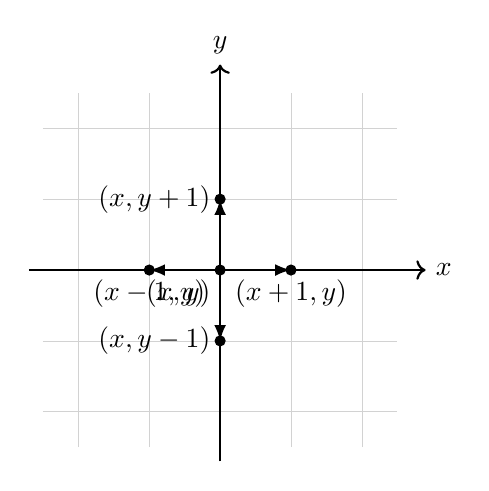
\begin{tikzpicture}[scale=0.9]
\draw[step=1cm, gray!35, very thin] (-2.5,-2.5) grid (2.5,2.5);
\draw[->, thick] (-2.7,0) -- (2.9,0) node[right] {$x$};
\draw[->, thick] (0,-2.7) -- (0,2.9) node[above] {$y$};

\filldraw[black] (0,0) circle (2pt) node[below left] {$(x,y)$};
\filldraw[black] (1,0) circle (2pt) node[below] {$(x+1,y)$};
\filldraw[black] (-1,0) circle (2pt) node[below] {$(x-1,y)$};
\filldraw[black] (0,1) circle (2pt) node[left] {$(x,y+1)$};
\filldraw[black] (0,-1) circle (2pt) node[left] {$(x,y-1)$};

\draw[-{Latex[length=2mm]}, thick] (0,0) -- (1,0);
\draw[-{Latex[length=2mm]}, thick] (0,0) -- (-1,0);
\draw[-{Latex[length=2mm]}, thick] (0,0) -- (0,1);
\draw[-{Latex[length=2mm]}, thick] (0,0) -- (0,-1);
\end{tikzpicture}
\end{center}

So from every point, there are four possible moves:
\[
\text{right, left, up, down}.
\]

\section{What Does Returning to the Origin Mean?}

Usually we start at
\[
S_0=(0,0).
\]

Returning to the origin after $n$ steps means
\[
S_n=(0,0).
\]

In probability notation:
\[
\Prob(S_n=(0,0)\mid S_0=(0,0)).
\]

This is the probability that the walker is back at the starting point after $n$ steps.

\section{Why Only Even Times Matter}

Just like in one dimension, a simple symmetric random walk on a grid can return to the starting point only after an even number of steps.

For example:
\[
\text{right, left}
\]
returns to the origin after 2 steps.

Also:
\[
\text{right, up, left, down}
\]
returns after 4 steps.

But after 1 step, the walker must be away from the origin. After 3 steps, it is also impossible to be exactly back at the origin.

So we study
\[
\Prob(S_{2n}=(0,0)\mid S_0=(0,0)).
\]

\section{The Key Result in Two Dimensions}

For the two-dimensional simple symmetric random walk,
\[
\Prob(S_{2n}=(0,0)\mid S_0=(0,0))
\sim
\frac{1}{\pi n}.
\]

This means that for large $n$, the return probability behaves approximately like
\[
\frac1{\pi n}.
\]

\subsection*{What Does $\sim$ Mean?}

The symbol
\[
\sim
\]
means ``asymptotically equal.''

So
\[
a_n\sim b_n
\]
means that for large $n$, $a_n$ behaves like $b_n$.

It does not mean they are exactly equal for every $n$.

\section{Why Does This Show Recurrence?}

The recurrence criterion says:
\[
\text{state }i\text{ is recurrent}
\quad\Longleftrightarrow\quad
\sum_{n=1}^{\infty}p_{ii}^{(n)}=\infty.
\]

For the origin $(0,0)$, this becomes:
\[
\sum_{n=1}^{\infty}
\Prob(S_n=(0,0)\mid S_0=(0,0)).
\]

Odd terms are zero, so we only look at even terms:
\[
\sum_{n=1}^{\infty}
\Prob(S_{2n}=(0,0)\mid S_0=(0,0)).
\]

Using the key result:
\[
\Prob(S_{2n}=(0,0)\mid S_0=(0,0))
\sim
\frac1{\pi n}.
\]

Therefore,
\[
\sum_{n=1}^{\infty}
\Prob(S_{2n}=(0,0)\mid S_0=(0,0))
\]
behaves like
\[
\sum_{n=1}^{\infty}\frac1{\pi n}.
\]

Since
\[
\frac1{\pi}
\]
is just a constant,
\[
\sum_{n=1}^{\infty}\frac1{\pi n}
=
\frac1{\pi}\sum_{n=1}^{\infty}\frac1n.
\]

The harmonic series diverges:
\[
\sum_{n=1}^{\infty}\frac1n=\infty.
\]

So
\[
\sum_{n=1}^{\infty}\frac1{\pi n}=\infty.
\]

Hence the two-dimensional simple symmetric random walk is recurrent.

\section{Why is it Null Recurrent?}

Recurrent means:
\[
\text{the walk returns to the origin eventually with probability }1.
\]

Positive recurrent means:
\[
\text{the expected return time is finite}.
\]

Null recurrent means:
\[
\text{the walk returns eventually, but the expected return time is infinite}.
\]

For the two-dimensional simple symmetric random walk:
\[
\text{return probability}=1,
\]
but the expected return time is infinite.

Therefore it is null recurrent.

\[
\boxed{\text{Two-dimensional simple symmetric random walk is null recurrent.}}
\]

\section{Three or More Dimensions}

In three dimensions, the state is
\[
S_n=(X_n,Y_n,Z_n).
\]

The walker moves in space, not just on a line or grid.

In higher dimensions, there are many more directions and many more places to go. So the walker has a greater chance of escaping far away and never returning to the origin.

The important result is:

\begin{corollary}
The simple symmetric random walk is recurrent for
\[
d=1,2
\]
and transient for
\[
d\geq 3.
\]
\end{corollary}

\section{Intuition: Why Dimension Matters}

\subsection*{One Dimension}

In one dimension, the walker is trapped on a line. If it moves far to the right, the only way to keep moving is still along the same line. It has many chances to cross the origin again.

\[
\boxed{d=1:\text{ recurrent}}
\]

\subsection*{Two Dimensions}

In two dimensions, the walker has more space to explore, but not enough to escape forever with positive probability. It still returns eventually with probability 1.

\[
\boxed{d=2:\text{ recurrent, but null recurrent}}
\]

\subsection*{Three or More Dimensions}

In three dimensions and higher, the walker has much more space to escape into. There is a positive probability that it never returns to the origin.

\[
\boxed{d\geq3:\text{ transient}}
\]

\section{Important Comparison Table}

\[
\begin{array}{c|c|c}
\text{Dimension} & \text{Behaviour} & \text{Meaning}\\
\hline
1 & \text{recurrent, null recurrent} & \text{returns eventually, infinite mean return time}\\
2 & \text{recurrent, null recurrent} & \text{returns eventually, infinite mean return time}\\
3\text{ or more} & \text{transient} & \text{may never return}
\end{array}
\]

\section{Worked Example 1}

\begin{example}
For a two-dimensional simple symmetric random walk starting at $(0,0)$, what are the possible states after one step?
\end{example}

\begin{answer}
From $(0,0)$, the walker can move:
\[
(1,0),\quad (-1,0),\quad (0,1),\quad (0,-1).
\]

Each occurs with probability
\[
\frac14.
\]
\end{answer}

\section{Worked Example 2}

\begin{example}
Can a two-dimensional simple symmetric random walk return to $(0,0)$ after 3 steps? Explain.
\end{example}

\begin{answer}
No. To return to the origin, the total number of moves must balance:
\begin{itemize}[leftmargin=1.2cm]
    \item right moves must equal left moves,
    \item up moves must equal down moves.
\end{itemize}

This requires an even number of total steps. Since 3 is odd, the walk cannot return to $(0,0)$ after 3 steps.

\[
\boxed{\Prob(S_3=(0,0)\mid S_0=(0,0))=0.}
\]
\end{answer}

\section{Worked Example 3}

\begin{example}
Using the approximation
\[
\Prob(S_{2n}=(0,0)\mid S_0=(0,0))\sim \frac1{\pi n},
\]
explain why the two-dimensional walk is recurrent.
\end{example}

\begin{answer}
The recurrence criterion says we look at
\[
\sum_{n=1}^{\infty}\Prob(S_{2n}=(0,0)\mid S_0=(0,0)).
\]

Using the approximation,
\[
\Prob(S_{2n}=(0,0)\mid S_0=(0,0))\sim \frac1{\pi n}.
\]

So the return-probability series behaves like
\[
\sum_{n=1}^{\infty}\frac1{\pi n}.
\]

Since
\[
\sum_{n=1}^{\infty}\frac1n=\infty,
\]
we also have
\[
\sum_{n=1}^{\infty}\frac1{\pi n}=\infty.
\]

Therefore the origin is recurrent. Since the chain is irreducible, all states are recurrent.
\end{answer}

\section{Practice Questions}

\begin{enumerate}[label=\textbf{Q\arabic*.}, leftmargin=1.2cm]
    \item What does
    \[
    S_n=(X_n,Y_n)
    \]
    mean in a two-dimensional random walk?

    \item What is the state space
    \[
    \mathbb{Z}^2?
    \]

    \item From state $(3,-2)$, list the four possible next states in a two-dimensional simple symmetric random walk.

    \item What is the probability of moving from $(x,y)$ to $(x,y+1)$ in a two-dimensional simple symmetric random walk?

    \item Can the walk return to the origin after 5 steps? Explain.

    \item What does
    \[
    \Prob(S_{2n}=(0,0)\mid S_0=(0,0))
    \]
    mean in words?

    \item If
    \[
    \Prob(S_{2n}=(0,0)\mid S_0=(0,0))\sim \frac1{\pi n},
    \]
    why does the corresponding series diverge?

    \item Is the two-dimensional simple symmetric random walk positive recurrent, null recurrent, or transient?

    \item What happens in dimensions $d\geq3$?

    \item Fill in the blanks:
    \[
    d=1,2 \Rightarrow \text{__________},
    \qquad
    d\geq3 \Rightarrow \text{__________}.
    \]
\end{enumerate}

\section{Answers}

\subsection*{Answer 1}

\[
S_n=(X_n,Y_n)
\]
means that the position at time $n$ is described by two coordinates.

$X_n$ is the horizontal coordinate, and $Y_n$ is the vertical coordinate.

\subsection*{Answer 2}

\[
\mathbb{Z}^2
\]
is the set of all ordered pairs of integers:
\[
\mathbb{Z}^2=\{(x,y):x,y\in\mathbb{Z}\}.
\]

It represents all grid points in two dimensions.

\subsection*{Answer 3}

From $(3,-2)$, the possible next states are:
\[
(4,-2),\quad (2,-2),\quad (3,-1),\quad (3,-3).
\]

\subsection*{Answer 4}

In a simple symmetric two-dimensional random walk, each of the four directions has probability
\[
\frac14.
\]

Therefore,
\[
\Prob((x,y)\to(x,y+1))=\frac14.
\]

\subsection*{Answer 5}

No. Returning to the origin requires moves to balance:
\[
\text{right}=\text{left},
\]
and
\[
\text{up}=\text{down}.
\]

So the total number of steps must be even. Since 5 is odd, returning after 5 steps is impossible.

\subsection*{Answer 6}

\[
\Prob(S_{2n}=(0,0)\mid S_0=(0,0))
\]
means the probability that the random walk is back at the origin after $2n$ steps, given that it started at the origin.

\subsection*{Answer 7}

The approximation says the return probabilities behave like
\[
\frac1{\pi n}.
\]

Thus the series behaves like
\[
\sum_{n=1}^{\infty}\frac1{\pi n}
=
\frac1{\pi}\sum_{n=1}^{\infty}\frac1n.
\]

The harmonic series
\[
\sum_{n=1}^{\infty}\frac1n
\]
diverges. Therefore the return-probability series also diverges.

\subsection*{Answer 8}

The two-dimensional simple symmetric random walk is recurrent but not positive recurrent.

Therefore, it is
\[
\boxed{\text{null recurrent}.}
\]

\subsection*{Answer 9}

For dimensions
\[
d\geq3,
\]
the simple symmetric random walk is transient.

This means there is a positive probability that the walk never returns to its starting point.

\subsection*{Answer 10}

\[
d=1,2 \Rightarrow \text{recurrent},
\]
\[
d\geq3 \Rightarrow \text{transient}.
\]

\end{document}
